\documentclass[a4paper, 12pt, final, garamond]{book}
\usepackage{cours-preambule}

\raggedbottom

\makeatletter
\renewcommand{\@chapapp}{\'Electrocin\'etique -- chapitre}
\makeatother

\begin{document}
\setcounter{chapter}{4}

\chapter{Correction du TD}

\section{Impédance équivalente}
\begin{enumerate}
    \item On commence par convertir le circuit avec les impédances complexes~:
        \begin{itemize}
            \item $\ul{Z}_{C_1} = \frac{1}{\jj C_1\w}$~;
            \item $\ul{Z}_L = \jj L\w$~;
            \item $\ul{Z}_{C_2} = \frac{1}{\jj C_2\w}$.
        \end{itemize}
        On peut ensuite déterminer l'impédance équivalente à l'association en
        parallèle de $L$ et $C_2$. Avec les admittances, on a
        \begin{gather*}
            \ul{Z}_{\eq,1}
                = \frac{1}{\frac{1}{\ul{Z}_{C_2}} + \frac{1}{\ul{Z}_L}}
                = \frac{1}{\jj C_2\w + \frac{1}{\jj L\w}}
                = \frac{\jj L\w}{1 - \w^2LC_2}
        \end{gather*}
        Il suffit alors de faire l'association en série de $\ul{Z}_{C_1}$ et de
        $\ul{Z}_{\eq,1}$~:
        \begin{gather*}
            \boxed{
            \ul{Z}_{\eq} = \jj C_1\w + \frac{\jj L\w}{1 - \w^2LC_2}}
        \end{gather*}
        Il n'est ici pas nécessaire d'aller plus loin dans le calcul.

    \item Ici, on utilise que $\ul{Z}_R = R$ et comme précédemment, on effectue
        l'association en parallèle des $R$ et $C$ de droite avant de faire
        l'association en série de $R$ et $C$ de gauche avec cette impédance
        équivalente~:
        \begin{gather*}
            \ul{Z}_{\eq, 1}
                = \frac{1}{\frac{1}{\ul{Z}_1} + \frac{1}{\ul{Z}_C}}
                = \frac{1}{\frac{1}{R} + \jj C\w}
                = \frac{R}{1 + \jj RC\w}
        \end{gather*}
        Et on a donc finalement
        \begin{gather*}
            \boxed{
            \ul{Z}_{\eq} = R + \frac{1}{\jj C\w} + \frac{R}{1 + \jj RC\w}}
        \end{gather*}
\end{enumerate}

\section{Circuit RL série en RSF}
\begin{enumerate}
    \item Pour les comportements limites, on utilise la modélisation d'une
        bobine à haute et basse fréquence~: étant donné que $\ul{Z}_L = \jj L
        \w$, pour $\w\rightarrow0$ on a $\ul{Z}_L = 0$, et pour
        $\w\rightarrow\infty$ on a $\ul{Z}_L \rightarrow \infty$. On a donc
        respectivement un fil et un interrupteur ouvert. En effet, l'impédance
        étant homogène à une résistance, une impédance nulle est semblable à une
        résistance nulle (un fil), et une impédance infinie est semblable à une
        résistance infinie (un interrupteur ouvert). \bigbreak
        Or, la tension d'un fil est nul, donc
        \[\boxed{u \xrightarrow[\w\rightarrow0]{} 0}\]
        Le courant ne peut traverser un interrupteur, donc en faisant la loi des
        mailles dans le circuit équivalent, on a $u_R = Ri = 0$, et forcément
        \[\boxed{u \xrightarrow[\w\rightarrow\infty]{} E}\]
    \item Pour cela, on utilise la relation du pont diviseur de tension~:
        \begin{gather*}
            \ul{U}
                = \frac{\ul{Z}_L}{\ul{Z}_L + \ul{Z}_R}E
            \Leftrightarrow
            \boxed{\ul{U}
            = \frac{\jj L\w}{R + \jj L \w}E}
        \end{gather*}

    \item La phase de $e(t)$ est nulle par construction. On calcule donc la
        phase de $u$ en prenant l'argument de son amplitude complexe~:

        \begin{gather*}
            \arg(\ul{U})
                = \arg(\jj L\w E) - \arg(R + \jj L \w)
                = \frac{\pi}{2} - \arctan \left( \frac{L\w}{R} \right)
        \end{gather*}
        où on peut prendre l'arctangente parce que la partie réelle est
        positive. Ainsi~:
        \begin{enumerate}
            \item Signaux en phase
                \begin{gather*}
                    \Leftrightarrow
                    \arg(\ul{U}) = 0
                    \Leftrightarrow
                    \arctan \left( \frac{L\w}{R} \right) = \frac{\pi}{2}
                    \Leftrightarrow
                    \boxed{\w \longrightarrow \infty}
                \end{gather*}
                C'est donc mathématiquement possible et physiquement
                approchable, mais pas rigoureusement.
            \item Signaux en opposition de phase
                \begin{gather*}
                    \Leftrightarrow
                    \arg(\ul{U}) = \pi
                    \Leftrightarrow
                    \arctan \left( \frac{L\w}{R} \right) = -\frac{\pi}{2}
                    \Leftrightarrow
                    \boxed{\w \longrightarrow -\infty}
                \end{gather*}
                C'est donc mathématiquement possible, mais \textbf{physiquement
                impossible}~: la pulsation est proportionnelle à la fréquence,
                et une fréquence ne saurait être négative.
            \item Signaux en quadrature de phase
                \begin{gather*}
                    \Leftrightarrow
                    \arg(\ul{U}) = \frac{\pi}{2}
                    \Leftrightarrow
                    \arctan \left( \frac{L\w}{R} \right) = 0
                    \Leftrightarrow
                    \boxed{\w = 0}
                \end{gather*}
                C'est donc possible à la fois mathématiquement et physiquement,
                mais cela correspond à un signal d'entrée qui ne varie pas,
                c'est-à-dire un régime permanent~: la sortie n'oscille donc pas
                non plus, et est simplement nulle. La quadrature de phase n'a
                donc pas vraiment de sens ici, la sortie est constamment nulle
                quand l'entrée est à son maximum.
        \end{enumerate}
\end{enumerate}

\section{Exploitation d'un oscillogramme en RSF}
\begin{enumerate}
    \item On lit l'amplitude de $e(t)$ à son maximum pour avoir \fbox{$E_m =
        \SI{10}{V}$}. On lit l'amplitude de $u(t)$ à son maximum pour avoir
        \fbox{$U_m = \SI{6}{V}$}. Pour la phase \textbf{à l'origine des temps},
        on regarde le signal à $t = 0$~: on lit $u(0) = U_m\cos(\f) =
        \SI{-3}{V}$, soit
        \begin{gather*}
            \boxed{\cos(\f) = \frac{u(0)}{U_m}}
            \qavec
            \left\{
                \begin{array}{rcl}
                    u(0) & = & \SI{-3}{V}\\
                    U_m & = & \SI{6}{V}
                \end{array}
            \right.\\
            \mathrm{A.N.~:}\quad
            \boxed{\f = \frac{2\pi}{3}\si{rad}}
        \end{gather*}
    \item On utilise un pont diviseur de tension pour avoir l'amplitude
        complexe~:
        \begin{gather*}
            \ul{U}
                = \frac{\ul{Z}_L}{\ul{Z}_R + \ul{Z}_C + \ul{Z}_L}E_m
                = \frac{1}{\frac{\ul{Z}_R}{\ul{Z}_L} + \frac{\ul{Z}_C}{\ul{Z}_L}
                + \frac{\ul{Z}_L}{\ul{Z}_L}}E_m
            \Leftrightarrow
            \ul{U}
                = \frac{1}{1 + \frac{R}{\jj L\w} + \frac{1}{\jj^2\w^2CL}}E_m\\
            \Leftrightarrow
            \boxed{
            \ul{U}
                = \frac{1}{1 -\jj \frac{R}{L\w} - \frac{1}{\w^2LC}}E_m
            }
        \end{gather*}
        On peut en vérifier l'homogénéité en se souvenant des résultats des
        chapitres précédents~:
        \begin{gather*}
            \w_0{}^2 = \frac{1}{LC}
            \qdonc
            \w^2LC \text{ adimensionné}
            \qet
            \frac{R}{L} = \tau^{-1}
            \qdonc
            \frac{R}{L\w} \text{ adimensionné}
        \end{gather*}
        D'une manière générale, on exprimera les résultats de la sorte, avec une
        fraction dont le numérateur est homogène à la quantité exprimée alors
        que le dénominateur est adimensionné. \bigbreak
        On trouve l'amplitude réelle en prenant le module de cette expression~:
        \begin{gather*}
            U_m
                = \left| \ul{U} \right|
            \Leftrightarrow
            \boxed{U_m
                = \frac{E}{\sqrt{\left(1 - \frac{1}{LC\w^2}\right)^2 +
                \frac{R^2}{L^2\w^2}}}
            }
        \end{gather*}
        On trouve la phase en en prenant l'argument~:
        \begin{gather*}
            \f
                = \arg(\ul{U})
                = \underbrace{\cancel{\arg(E)}}_{=0}
                    - \arg \left( 1 - \frac{1}{LC\w^2} - \jj \frac{R}{L\w}
                    \right)\\
            \Leftrightarrow
            \tan(\f)
                = - \left(-\frac{R}{L\w}\times \frac{1}{1 - \frac{1}{LC\w^2}}\right)
                = \frac{R}{L\w - \frac{1}{C\w}}
            \Leftrightarrow
            \boxed{\tan(\f)
                = \frac{RC\w}{LC\w^2 - 1}
            }
        \end{gather*}
        Ici, il n'est pas évident de prendre l'arctangente de la tangente~: la
        partie réelle de l'argument calculé n'est pas forcément positif (il
        l'est si $\w^2 > \frac{1}{LC}$).
    \item Il paraît évidemment plus simple de calculer $L$ à partir de la phase,
        sachant qu'on a déterminé $\f$ à la première question~:
        \begin{gather*}
            LC\w^2 - 1
                = \frac{RC\w}{\tan(\f)}
            \Leftrightarrow
            LC\w^2 = 1 + \frac{RC\w}{\tan(\f)}\\
            \Leftrightarrow
            \boxed{L = \frac{1}{C\w^2} + \frac{R}{\w\tan(\f)}}
            \qavec
            \left\{
                \begin{array}{rcl}
                    C  & = & \SI{0.10}{\micro F}\\
                    \w & = & 2\pi f\\
                    f  & = & \SI{1.2e3}{Hz}\\
                    R  & = & \SI{1}{k\Omega}\\
                    \f & = & \frac{2\pi}{3}\si{rad}
                \end{array}
            \right.\\
            \mathrm{A.N.~:}\quad
            \boxed{L = \SI{9.9e-2}{H}}
        \end{gather*}
\end{enumerate}

\section{Comportement d'un circuit à haute et basse fréquences}
\begin{enumerate}
    \item On utilise la relation pour passer des réels aux complexes, pour avoir
        \[
            \boxed{\ul{e}(t) = E_m\exr^{\jj\wt}}
            \qet
            \boxed{\ul{u}(t) = U_m\exr^{\jj(\wt+\f)}}
        \]
        Pour avoir les amplitudes complexes, on sépare le terme en $\wt$ du
        terme de phase~: on trouve donc
        \[
            \boxed{\ul{E} = E_m}
            \qet
            \boxed{\ul{U} = U_m\exr^{\jj\f}}
        \]
    \item 
    S'il n'y avait pas la capacité, on pourrait facilement utiliser un pont
    diviseur de tension pour exprimer $\ul{u}$ en fonction de $\ul{e}$,
    $\ul{Z}_R$ et $\ul{Z}_L$. Pour se ramener à la situation du pont diviseur de
    tension, on détermine donc une première impédance équivalente issue de
    l'association en parallèle de $L$ et $C$, après les avoir converties en
    complexes. \bigbreak
    On peut déterminer $\ul{Z}_{\eq, 1}$ avec les admittances $\ul{Y}_L = 1/\jj
    L \w$ et $\ul{Y}_C = \jj C\w$, et utiliser le pont diviseur de tension
    directement avec l'amplitude complexe~: $\ul{U} =
    \frac{\ul{Z}_{\eq,1}}{\ul{Z}_{\eq,1}+\ul{Z}_R}E_m$. Ainsi,
    \begin{gather*}
        \ul{U} = \frac{\dfrac{1}{
            \color{orange}\cancel{\dfrac{1}{\jj L\w} + \jj C\w}}}
            {\dfrac{1}{\textcolor{orange}{\cancel{\dfrac{1}{\jj L\w} + \jj C\w}}}
            + R\color{orange}(…)}E_0
            \times \textcolor{orange}{
                \frac{\jj C\w + \dfrac{1}{\jj L\w}}{\jj C\w + \dfrac{1}{\jj L\w}}}
        \Leftrightarrow
        \ul{U} = \frac{1}{1 + \jj RC\w + \dfrac{R}{\jj L\w}}E_0\\
        \Leftrightarrow
        \boxed{
            \ul{U} = \frac{E_0}{1 + \jj \left( RC\w - \dfrac{R}{L\w} \right)}
        }
    \end{gather*}
    où on a simplifié la fraction en multipliant par le terme orange d'abord,
    puis en utilisant que $1/\jj = -\jj$.
    \item On trouve l'amplitude réelle en prenant le module de l'amplitude
        complexe, et la phase en en prenant l'argument~:
        \begin{gather*}
            U_m
                = \left| \ul{U} \right|
            \Leftrightarrow
            \boxed{U_m
                = \frac{E_m}{\sqrt{1 + \left( RC\w - \dfrac{R}{L\w} \right)^2}}
            }\\
            \f
                = \underbrace{\cancel{\arg(E_m)}}_{=0}
                    - \arg \left( 1 + \jj \left( RC\w - \dfrac{R}{L\w} \right) \right)
            \Leftrightarrow
            \tan\f = - \frac{RC\w - \dfrac{R}{L\w}}{1}\\
            \Leftrightarrow
            \boxed{\f = \arctan \left( RC\w - \frac{R}{L\w} \right)}
        \end{gather*}

    \item À très haute fréquence, i.e.\ $\w\rightarrow\infty$, le dénominateur
        de l'amplitude réelle tend vers l'infini à cause du terme $RC\w$, donc
        l'amplitude vers 0~; c'est la même chose à très basse fréquence, i.e.\
        $\w\rightarrow0^+$~: le dénominateur tend vers l'infini et l'amplitude
        vers 0, mais cette fois à cause du terme en $\dfrac{R}{L\w}$. On a donc
        \[
            \boxed{U_m \xrightarrow[\w\rightarrow\infty]{} 0}
            \qet
            \boxed{U_m \xrightarrow[\w\rightarrow0^+]{} 0}
        \]
        On pouvait prévoir ces résultats par l'étude directe du montage et des
        impédances en jeu~: en effet,
        \begin{align*}
            \ul{Z}_C
                = \frac{1}{\jj C\w}
            \Rightarrow
            |\ul{Z}_C| \xrightarrow[\w\rightarrow0]{} \infty
            &\qet
            |\ul{Z}_C| \xrightarrow[\w\rightarrow\infty]{} 0\\
            \ul{Z}_L
                = \jj L\w
            \Rightarrow
            |\ul{Z}_L| \xrightarrow[\w\rightarrow0]{} 0
            &\qet
            |\ul{Z}_L| \xrightarrow[\w\rightarrow\infty]{} \infty
        \end{align*}
        Dans les deux cas, le circuit équivalent est l'association en série
        d'une résistance avec une association en parallèle d'un interrupteur
        ouvert et d'un fil, c'est-à-dire un fil~: or, la tension d'un fil est
        nulle.
\end{enumerate}

\section{Dipôle inconnu}
\begin{enumerate}
    \item On trouve les amplitudes par lecture graphique des maxima~:
        \[
            \boxed{V_m = \SI{3.5}{V}}
            \qet
            \boxed{U_m = \SI{5}{V}}
        \]
        On fait de même pour trouver la période $T = \SI{6.3e-2}{s}$, et on en
        déduit la pulsation~:
        \[\boxed{\w = \frac{2\pi}{T} = \SI{100}{rad.s^{-1}}}\]
    \item La tension $v$ est en $avance$ sur $u$, puisque quand $v$ s'annule en
        descendant $u$ s'annule aussi en descendant un peu plus tard que $v$. On
        peut aussi voir qu'à $t=0$, $u$ est à son maximum alors que $v$ y est
        déjà passé et est en train de diminuer. Par définition du déphasage, on
        a donc \fbox{$\D\f_{v/u} > 0$}. \bigbreak
        Or, $\D\f_{v/u} = \f_v - \f_u$ et $u(t) = U_m\cos(\wt)$ donc $\f_u = 0$.
        On trouve donc \fbox{$\F > 0$}. \bigbreak
        On a deux manières de mesurer le déphasage~:
        \begin{itemize}
            \item par définition, la pulsation est une vitesse angulaire, donc
                une durée se convertit en phase en la multipliant par $\w$. On
                peut donc déterminer le \textbf{déphasage} en mesurant le
                \textbf{retard temporel} entre les deux signaux \textbf{quand
                ils s'annulent avec la même pente}. Soit $\D t$ cet écart~: on
                mesure
                \begin{gather*}
                    \D t = \SI{0.75e-2}{s}
                    \Leftrightarrow
                    \D\f_{v/u} = \F = \w\D t
                    \Leftrightarrow
                    \boxed{\F = \SI{0.75}{rad} \approx \frac{\pi}{4}\si{rad}}
                \end{gather*}
            \item On peut également mesurer $v(0) = V_m\cos(\F)$ et avoir
                \begin{gather*}
                    \cos(\F) = \frac{v(0)}{V_m}
                    \Leftrightarrow
                    \boxed{\F = \arccos \left( \frac{v(0)}{V_m} \right)}
                    \qavec
                    \left\{
                        \begin{array}{rcl}
                            v(0) & = & \SI{2.5}{V}\\
                            V_m & = & \SI{3.5}{V}
                        \end{array}
                    \right.\\
                    \mathrm{A.N.~:}\quad
                    \boxed{\F \approx \SI{0.77}{rad}}
                \end{gather*}
        \end{itemize}
    \item
        \begin{enumerate}
            \item On nous donne $v(t)$ donc $\ul{V} = V_m\exr^{\jj\F}$, et on
                nous défini $\ul{Z}$ son impédance. Pour faire le lien entre
                les deux, on utilise la définition de l'impédance complexe pour
                un dipôle de tension $\ul{U}$ et traversé par un courant
                $\ul{I}$ \textit{via} loi \textbf{loi d'Ohm généralisée}~:
                \[\boxed{\ul{V} = \ul{Z}\ul{I}}\]
                Il faudrait donc pouvoir connaître $\ul{I}$. Heureusement, la
                loi d'\textsc{Ohm} généralisée fonction évidemment avec les
                résistances, et comme il n'y a qu'une seule intensité qui
                traverse la maille, on peut utiliser
                \[\boxed{\ul{U} = R\ul{I} \Leftrightarrow \ul{I} =
                \frac{\ul{U}}{R}}\]
                Ainsi,
                \begin{gather*}
                    Z = \left| \ul{Z} \right| = \sqrt{X^2 + Y^2} \qet
                    Z = \left| \ul{Z} \right| = \left| \frac{\ul{V}}{\ul{I}} \right|
                    = \left| R\frac{\ul{V}}{\ul{U}} \right|\\
                    \Leftrightarrow
                    \boxed{X^2 + Y^2 = R^2 \frac{V_m{}^2}{U_m{}^2}}
                    \qavec
                    \left\{
                        \begin{array}{rcl}
                            V_m & = & \SI{3.5}{V}\\
                            U_m & = & \SI{5}{V}\\
                            R   & = & \SI{100}{\Omega}
                        \end{array}
                    \right.\\
                    \mathrm{A.N.~:}\quad
                    \boxed{X^2 + Y^2 = \SI{4900}{\Omega^2}}
                \end{gather*}
                L'autre équation permettant de résoudre ce système est bien
                évidemment la phase (question 1 puis question 2)~:
                \begin{gather*}
                    \tan(\arg(\ul{Z})) = \frac{Y}{X} \qet \tan(\arg(\ul{Z})) =
                    \tan(\arg(\ul{V}) -
                    \underbrace{\cancel{\arg(\ul{U})}}_{=0}) = \tan(\F)\\
                    \Leftrightarrow
                    \frac{Y}{X} = \tan\F
                    \qavec
                    \F = \frac{\pi}{4}\si{rad}
                    \qsoit
                    \boxed{\frac{Y}{X} = 1}
                \end{gather*}
                On combine les deux équations pour trouver
                \begin{gather*}
                    Y = X
                    \qet
                    2X^2 = \SI{3900}{\Omega^2}\\
                    \mathrm{A.N.~:}\quad
                    \boxed{X = Y = \SI{49}{\Omega}}
                \end{gather*}
            \item La partie réelle est non nulle, donc on a au moins une
                résistance de $\SI{49}{\Omega}$, et la partie imaginaire est
                positive~: ça ne peut qu'être une inductance car $1/\jj C\w =
                -\jj/C\w$ et la partie imaginaire est donc négative. C'est donc
                \textbf{l'association en série d'une résistance $r$ et d'une
                inductance $L$}. On trouve
                la valeur de $L$ en calculant $L\w = Y = \SI{49}{\Omega}$.
                \[
                    \boxed{r = \SI{49}{\Omega}}
                    \qet
                    \boxed{L = \SI{0.49}{H}}
                \]
        \end{enumerate}
\end{enumerate}

\section{Obtention d'une équation différentielle}
On nomme les tensions et intensités dans le circuit, et on utilise la loi des
nœuds et la loi d'Ohm généralisée~:

\begin{minipage}{0.70\linewidth}
    \begin{gather}
        \nonumber
        \ul{I} = \ul{I_1} + \ul{I_2}\\
        \nonumber
        \Leftrightarrow
        \frac{1}{R}\ul{U_R} = \frac{1}{\ul{Z}_{2C}}\ul{U'} + \frac{1}{\ul{Z}_C}\ul{U}\\
        \label{eq:ex6}
        \Leftrightarrow
        \ul{U_R} = 2\jj RC\w\ul{U'} + \jj RC\w\ul{U}
    \end{gather}
\end{minipage}
\begin{minipage}{0.30\linewidth}
    \centering
    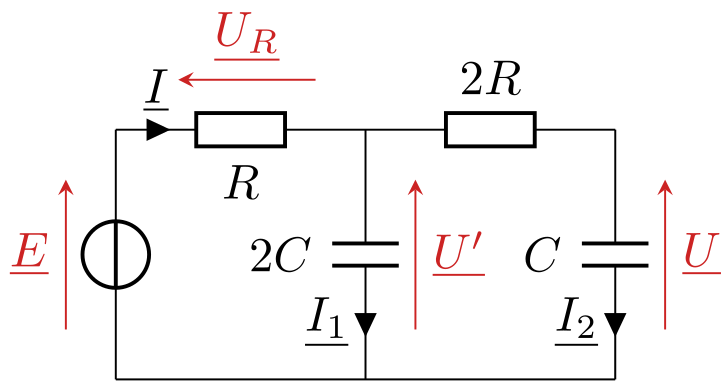
\includegraphics[width=\linewidth]{exo6_solve}
\end{minipage}
On utilise ensuite la loi des mailles à droite et à gauche, donnant
respectivement~:
\begin{gather*}
    \ul{U'} = \ul{U} + 2R\ul{I_2} = \ul{U} + 2\jj RC\w\ul{U}
    \qet
    \ul{U_R} = \ul{E} - \ul{U'} = \ul{E} - \ul{U} - 2\jj RC\w\ul{U}
\end{gather*}
On regroupe les équations dans \ref{eq:ex6} et on introduit $\tau = RC$~:
\begin{gather*}
    \ul{E} - \ul{U} - 2\jj\w\tau\ul{U} = \jj\w\tau \left( \ul{U} +
    2\jj\w\tau\ul{U} \right) + \jj\w\tau\ul{U}\\
    \Leftrightarrow
    \ul{E} = \ul{U} + 5\jj\w\tau\ul{U} + 4\tau^2 (\jj\w)^2\ul{U}
\end{gather*}
En identifiant les puissances de $\jj\w$ à l'ordre des dérivées pour retourner
dans le domaine des représentations réelles, on a donc bien
\begin{gather*}
    \boxed{
        e = u + 5\tau \dv{u}{t} + 4\tau^2 \dv[2]{u}{t}}
\end{gather*}
\relax
\section{Déphasage, pulsation et impédance}

Pour exprimer simplement $i$, il nous faut une seule maille avec une seule
impédance équivalente $\ul{Z}_{\eq}$~: de cette manière, la loi des mailles nous
donnera $\ul{E} = \ul{Z}_{\eq}\ul{I}$ et on pourra facilement déterminer le
déphasage entre $i$ et $e$. \bigbreak
On calcule l'impédance équivalente de l'association en série de $R_2$ et $L$~:
\[\ul{Z}_{\eq,1} = R_2 + \jj L\w\]
Cette association est en parallèle avec $C$~:
\begin{gather*}
    \ul{Z}_{\eq, 2}
        = \frac{\ul{Z}_C\times\ul{Z}_{\eq, 1}}{\ul{Z}_C + \ul{Z}_{\eq,1}}
        = \frac{\dfrac{1}{\jj C\w}(R_2 + \jj L\w)}{\dfrac{1}{\jj C\w} + R_2 +
            \jj L\w}\\
    \Leftrightarrow
    \ul{Z}_{\eq,2} = \frac{R_2 + \jj L\w}{1+\jj R_2C\w - LC\w^2}
\end{gather*}
On a donc comme prévu avec la loi des mailles~:
\[\boxed{\ul{I} = \frac{\ul{E}}{R_1 + \ul{Z}_{\eq,2}}}\]
L'intensité est en phase avec la tension si $\arg(R_1 + \ul{Z}_{\eq,2}) = 0$,
c'est-à-dire si
\begin{align*}
    \arg\left(R_1 + \frac{R_2 + \jj L\w}{1 + \jj R_2C\w - LC\w^2}\right)
        &= 0\\
    \Leftrightarrow
    \arg \left( \frac{R_1 + \jj R_1R_2C\w - LCR_1\w^2 + R_2 + \jj L\w}
        {1 + \jj R_2 C\w - LC\w^2} \right)
        &= 0\\
    \Leftrightarrow
    \arg \left( (R_1 + R_2 - LCR_1\w^2) + \jj(R_1R_2C\w + L\w) \right)
        & = \arg \left( (1-LC\w^2) + \jj R_2C\w \right)\\
    \Leftrightarrow
    \tan \left(\arg \left( (R_1 + R_2 - LCR_1\w^2) + \jj(R_1R_2C\w + L\w) \right)\right)
        & = \tan\left(\arg \left( (1-LC\w^2) + \jj R_2C\w \right)\right)\\
    \Leftrightarrow
    \frac{R_1R_2C\w + L\w}{R_1 + R_2 - LCR_1\w^2}
        &= \frac{R_2C\w}{1-LC\w}\\
    \Leftrightarrow
    \frac{R_1 + \dfrac{L\cancel{\w}}{R_2C\cancel{\w}}}{R_1 + R_2 - LCR_1\w^2}
        &= \frac{1}{1-LC\w^2}\\
    \Leftrightarrow
    \left( R_1 + \frac{L}{R_2C} \right) \left( 1-LC\w^2 \right)
        &= R_1 + R_2 - LCR_1\w^2\\
    \Leftrightarrow
    \cancel{R_1} - \bcancel{LCR_1\w^2} + \frac{L}{R_2C} - \frac{L^2\w^2}{R_2}
        &= \cancel{R_1} + R_2 - \bcancel{LCR_1\w^2}\\
    \Leftrightarrow
    L
        &= R_2{}^2 C + L^2C\w^2\\
    \Leftrightarrow
    \w^2
        &= \frac{1}{LC} - \frac{R_2{}^2}{L^2}\\
    \Leftrightarrow
    \Aboxed{\w^2
        &= \frac{1}{LC} \left( 1 - \frac{R_2{}^2C}{L} \right)}
\end{align*}

\section{Oscillateur à quartz}
\begin{enumerate}
    \item On calcule l'association en série de $C$ et $L$ d'abord, puis on fait
        l'association en parallèle de ce dipôle avec $C_0$~:
        \begin{gather*}
            \ul{Z}_{\eq, 1} = \frac{1}{\jj C\w} + \jj L \w
        \end{gather*}
        D'où
        \begin{align*}
            \ul{Z}
                &= \frac{1}{\ul{Y}_{C_0} + \ul{Y}_{\eq, 1}}\\
            \Leftrightarrow
            \ul{Z}
                &= \frac{1}{\jj C_0\w + \dfrac{1}{\frac{1}{\jj C\w} + \jj L\w}}
                \times
                \frac{\frac{1}{\jj C\w} + \jj L\w}{\frac{1}{\jj C\w} + \jj
                L\w}\\
            \Leftrightarrow
            \ul{Z}
                &= \frac{\frac{1}{\jj C\w} + \jj L\w}{1 + \frac{C_0}{C} -
                LC_0\w^2}
                \times
                \frac{\jj C\w}{\jj C\w}\\
            \Leftrightarrow
            \ul{Z}
                &= \frac{1 - LC\w^2}{\jj C\w + \jj C_0\w -\jj LCC_0\w^3}\\
            \Leftrightarrow
            \ul{Z}
                &= -\jj \frac{1 - LC\w^2}{(C+C_0)\w - LCC_0\w^3}\\
            \Leftrightarrow
            \Aboxed{\ul{Z}
                &= \jj \frac{LC\w^2 - 1}{\w\left((C+C_0) - LCC_0\w^2\right)}}
        \end{align*}
    \item L'impédance est nulle si le numérateur est nul, c'est-à-dire
        \[\boxed{\ul{Z} = 0 \Leftrightarrow \w = \w_0 = \sqrt{\frac{1}{LC}}}\]
        À cette pulsation, assimilable à la pulsation propre d'un circuit RLC
        série, le dipôle est donc équivalent à un fil. On retrouvera ce
        résultat en étudiant la résonance dans le chapitre suivant. \bigbreak
        L'impédance est infinie si le dénominateur est nul, c'est-à-dire
        \[\boxed{|\ul{Z}| \rightarrow \infty \Leftrightarrow \w = \w_0' =
            \sqrt{\frac{C+C_0}{LCC_0}}}\]
        Cette pulsation serait la pulsation propre d'une bobine $L$ et d'un
        condensateur de capacité $C_{\eq} = \frac{CC_0}{C+C_0}$, autrement dit
        l'association en série d'un condensateur $C$ et d'un autre condensateur
        $C_0$ (les inverses des capacités s'ajoutent en série). \smallbreak
        À cette pulsation (dite «~de résonance~», cf.\ chapitre suivant), la
        bobine et les condensateurs se chargent et déchargent alternativement,
        l'énergie arrivant dans le dipôle est piégée et n'a pas transmise au
        reste du circuit, comme le fait un interrupteur ouvert.
    \item~

        \begin{minipage}{0.60\linewidth}
            On regarde les cas limites à très haute et très basse fréquence~:
            \begin{gather*}
                |\ul{Z}| \xrightarrow[\w\rightarrow\infty]{} 0
                \qet
                |\ul{Z}| \xrightarrow[\w\rightarrow0^+]{} \infty
            \end{gather*}
            En effet, à $\w \rightarrow 0$, les condensateurs sont des interrupteurs
            ouverts donc l'impédance totale est celle d'un interrupteur ouvert. À
            l'inverse, à $\w \rightarrow \infty$, les condensateurs sont des fils
            donc l'impédance totale est celle d'un fil~: 0.
        \end{minipage}
        \hfill
        \begin{minipage}{0.45\linewidth}
            \begin{center}
                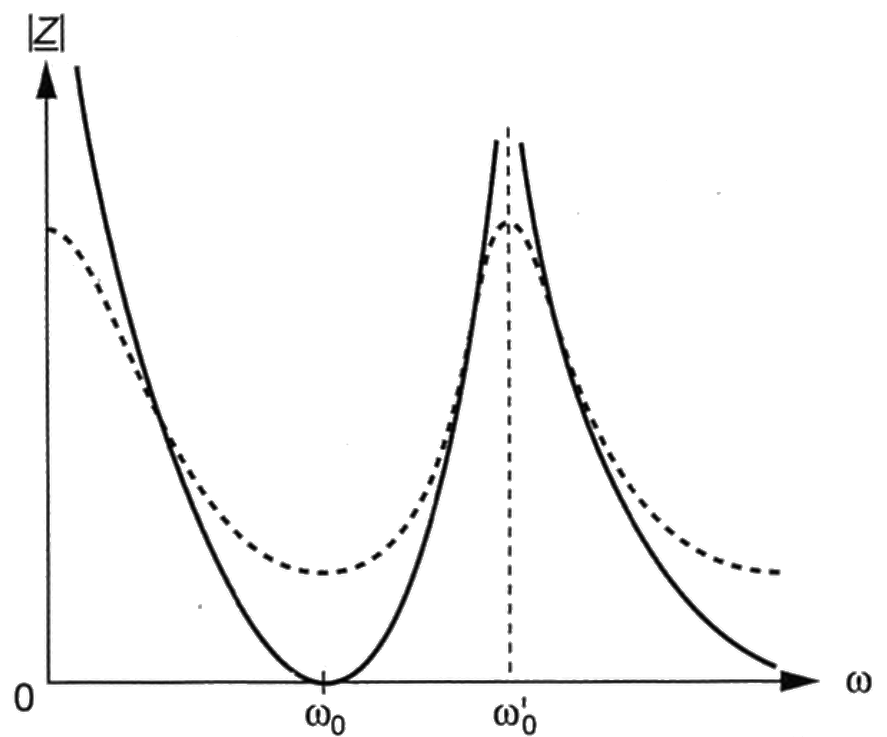
\includegraphics[width=\linewidth]{exo8_solve-clean}
            \end{center}
        \end{minipage}
    \item Les résistances évitent les infinités par dissipation, mais également
        les valeurs nulles~: on se retrouve avec la courbe en pointillés sur la
        figure précédente.
\end{enumerate}

\end{document}
